\documentclass[10pt,a4paper]{ctexart}

% Compile with XeLaTeX. Compact two-column midterm summary.
\usepackage[a4paper,margin=0.30in,includeheadfoot]{geometry}
\usepackage{amsmath,amssymb,mathtools}
\usepackage{siunitx}
\usepackage{multicol}
\usepackage{booktabs,tabularx,array}
\usepackage{enumitem}
\usepackage{titlesec}
\usepackage{xcolor}
\usepackage{microtype}
\usepackage{fancyhdr}
\usepackage[hidelinks]{hyperref}

\pagestyle{fancy}
\fancyhf{}
\fancyfoot[C]{\small\thepage}
\setlength{\headheight}{5pt}
\setlength{\headsep}{2pt}
\setlength{\footskip}{12pt}
\setlength{\columnsep}{0.14in}
\setlength{\columnseprule}{0.2pt}
\setlength{\parindent}{0pt}
\setlength{\parskip}{0.5pt}
\linespread{0.91}
\emergencystretch=2em

\AtBeginDocument{\fontsize{10pt}{9.1pt}\selectfont}
\titleformat{\section}{\normalsize\bfseries\color{blue!55!black}}{}{0pt}{}
\titlespacing*{\section}{0pt}{2pt}{0.5pt}
\titleformat{\subsection}{\normalsize\bfseries\color{black!75}}{}{0pt}{}
\titlespacing*{\subsection}{0pt}{1.5pt}{0pt}
\titleformat{\subsubsection}{\small\bfseries}{}{0pt}{}
\titlespacing*{\subsubsection}{0pt}{1pt}{0pt}
\setlist{nosep,leftmargin=*,topsep=0.5pt,partopsep=0pt}
\setlist[itemize]{label=\textbullet}
\setlist[enumerate]{label=\arabic*.,labelsep=0.3em}

\newcommand{\key}[1]{\textbf{#1}}
\newcommand{\formula}[1]{%
	\par\vspace{1pt}\begingroup
	\setlength{\abovedisplayskip}{0pt}\setlength{\belowdisplayskip}{0pt}
	\[ #1 \]\endgroup\vspace{1pt}}
\newcolumntype{Y}{>{\raggedright\arraybackslash}X}

\begin{document}
\begin{multicols*}{2}
\sloppy

\section{1. Biochips and System Design}
\subsection{Biochip concept}
\begin{itemize}
	\item Biochip is a compact platform that integrates biological or biochemical functions with microtechnology, 
	sensing and data output.
	\item Biochip core principle include biological function, microtechnology, signal detection and user workflow.
	\item Biochip is a bundle as biology + engnieering + information which packaged for a user.
\end{itemize}

\subsection{Core terminology}
\begin{itemize}
	\item \key{MEMS}: short for 'Microelectromechanical Systems', microfabricated structures + electrical/mechanical components, 
	sensors, actuators and control circuits.
	\item \key{BioMEMS:} MEMS applied to biology, medicine and healthcare; e.g. microfluidics, cell culture, electrode arrays.
	\item \key{Biochip:} compact platform integrating biological/analytical functions, fluidics, sensing, electronics and output.
	\item \key{Biosensor:} biological recognition element + transducer + signal processing/readout.
	\item \key{Lab-on-a-chip:} miniaturized laboratory workflow using small volumes: sample preparation, reaction, separation, 
	detection and analysis.\\
	\makebox[\linewidth][c]{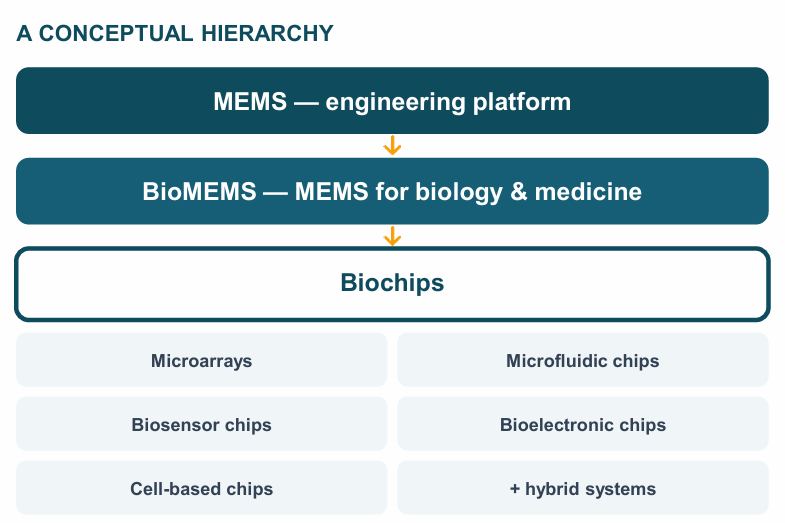
\includegraphics[width=0.5\linewidth]{Relationship.png}}
\end{itemize}

\subsection{Signal and functional architecture}
\begin{itemize}
	\item Recognition \(\rightarrow\) physical/chemical change \(\rightarrow\) transduction \(\rightarrow\) measurable output.
	\item Sample input \(\rightarrow\) preparation \(\rightarrow\) separation/concentration \(\rightarrow\) reaction/recognition \(\rightarrow\) detection \(\rightarrow\) signal processing \(\rightarrow\) data output.
	\item Supporting modules: reagent storage, fluid control, temperature control, waste handling and quality control.
	\item Detection: fluorescence, absorbance, chemiluminescence, colour, electrochemical current, impedance or displacement.
\end{itemize}

\subsection{Integration versus automation}
\begin{itemize}
	\item \key{Integration}: connect multiple functions in one system.
	\item \key{Automation}: reduce manual intervention using pumps, valves, temperature control, imaging and software.
	\item They are independent: a device may be integrated but manual, or automated but not fully integrated.
\end{itemize}

\subsection{Miniaturization}
\begin{itemize}
	\item Benefits: lower sample/reagent use, shorter transport distance, faster heat transfer, faster analysis, portability, automation and throughput.
	\item Limitations: clogging, bubbles, evaporation, adsorption, lower absolute signal, fabrication/packaging complexity and device variation.
	\item \key{Design rule}: optimize the complete system: performance + reliability + usability + manufacturability, not size alone.
\end{itemize}

\subsection{Design workflow}
\begin{enumerate}
	\item Define biomedical need and user.
	\item Define target, sample matrix, concentration, interferents, sensitivity and specificity.
	\item Select assay and device category.
	\item Map sample-to-answer architecture; separate on-chip, off-chip, manual and automated functions.
	\item Co-design material, fabrication and detection.
	\item Package, test, validate in the real use environment and redesign.
\end{enumerate}
\textit{Biology sets requirements; engineering sets constraints.}


\section{2. Scaling and Micro-Scale Physics}
\subsection{Geometric scaling}
\begin{itemize}
	\item If every length scales by \(s\): \(L\propto s\), \(A\propto s^2\), \(V\propto s^3\), therefore \(A/V\propto1/s\).
	\item Smaller devices have relatively more surface: adsorption, wetting, surface charge, wall friction, evaporation and heat exchange become important.
	\item Hydraulic diameter: \(D_H=4A/P\).
\end{itemize}

\subsection{Flow and hydraulic resistance}
\begin{itemize}
	\item For a Newtonian fluid, \(\tau=\mu\,du/dy\). Circular-channel Hagen--Poiseuille flow:
\end{itemize}
\formula{\begin{aligned}
Q&=\frac{\pi R^4\Delta P}{8\mu L},& Q&=\frac{\Delta P}{R_h}, &R_h=\frac{8\mu L}{\pi R^4}.
\end{aligned}}
\begin{itemize}
	\item For a shallow rectangular channel, \(R_h\propto\mu L/(wh^3)\): height errors strongly affect flow. 
	Series resistances add; parallel channels reduce resistance.
\end{itemize}

\subsection{Dimensionless numbers}
\begin{itemize}
	\item Reynolds number compares inertia with viscosity, discribe how fliud action
\end{itemize}
\formula{\mathrm{Re}=\frac{\rho UL}{\mu}}
\begin{itemize}
	\item Low Re: viscosity dominates, smooth laminar and nearly reversible flow; high Re: inertia matters and turbulence may occur. 
	Microfluidics often has \(\mathrm{Re}<100\), frequently \(<1\).\\
	\makebox[\linewidth][c]{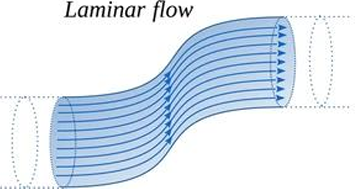
\includegraphics[width=0.5\linewidth]{LaminarFlow.png}}
	\item There are usually two modes of flow in nature. Laminar flow usually occurs with smooth streamlines, limited cross-stream mixing, 
	predictable velocity profiles, low flow instability and strong dependence on viscosity.\\
	\makebox[\linewidth][c]{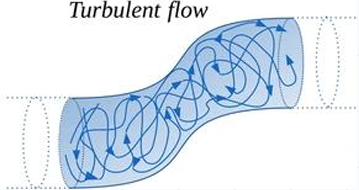
\includegraphics[width=0.5\linewidth]{TurbulentFlow.png}}\\
	While on contrast, turbulent flow typically shows like random fluctuations, strong mixing, large vortices and higher energy dissipation.\\
	\item If a fluid at low Re, its inertia is negligible; flow is highly viscous; reversing the pressure reverses the flow; 
	mixing by chaotic advection is difficult; geometry and diffusion become critical. Hence designers therefore rely on diffusion, 
	channel geometry, chaotic advection or active mixing.
	\item \key{Mix two viscous components:}\\
	According to definition of Re, it should increase the flow rate, include mixing geometry or mix components by leapfrogging transport.
\end{itemize}

\subsection{Diffusion and mixing}
\begin{itemize}
	\item Diffusion is molecular transport caused by random thermal motion, 
	molecules move from regions of high concentration to regions of low concentration.
	\item Diffusion can be described by Fick's law, so as diffustion time $t_D$:
\end{itemize}
\formula{\begin{aligned}
\text{Fick first law:} & J=-D\frac{dC}{dx},\\
\text{Fick second law:} & \frac{\partial C}{\partial t}=D\frac{\partial^2C}{\partial x^2},\\
\rightarrow t_D&\sim\frac{L^2}{D}.
\end{aligned}}
\begin{itemize}
	\item Reducing the diffusion distance by 10 reduces diffusion time by 100. Low-Re streams remain side-by-side; 
	use narrower channels, longer residence, serpentine/herringbone structures, droplets or active mixing.
	\item Péclet Number shows whether molecules are carried downstream by bulk flow faster than they diffuse across the channel.
\end{itemize}
\formula{\mathrm{Pe}=\frac{UL}{D}}
\begin{itemize}
	\item Low Pe: diffusion dominates. High Pe: advection carries material downstream faster than cross-stream diffusion; 
	fast transport but difficult mixing.
\end{itemize}

\subsection{Interfaces and droplets}
\begin{itemize}
	\item Surface tension arises from cohesive intermolecular forces acting at an interface between two phases.
	\item Surface tension generally measure by Young–Laplace pressure, which are following:\\
\end{itemize}
\formula{\begin{aligned}
\text{Curved interface:} \Delta P&=\gamma\left(\frac1{R_1}+\frac1{R_2}\right),
\end{aligned}}
\formula{\begin{aligned}
\text{Spherical droplet:} \Delta P_{\mathrm{sphere}}&=\frac{2\gamma}{R},
\end{aligned}}
\formula{\begin{aligned}
\text{Capillary channel:} \Delta P_c&\approx\frac{2\gamma\cos\theta}{r}.
\end{aligned}}
\begin{itemize}
	\item Hydrophilic (small \(\theta\)): aqueous filling promoted. 
	Hydrophobic (large \(\theta\)): filling resisted and air trapping possible.
	\item Capillary number compares viscous stress with surface tension, and indicates whether flow deforms interfaces.
\end{itemize}
\formula{\mathrm{Ca}=\frac{\mu U}{\gamma}}
\begin{itemize}
	\item Low Ca: surface tension controls shape; high Ca: viscous stress deforms interfaces. 
	Droplet size depends on flow-rate ratio, geometry, viscosity ratio, wettability, surfactant and Ca.
	\item There are many other important dimensionless numbers like:\\
	\key{Womersley number:} measure unsteady inertial effect, \(\mathrm{Wo}=L\sqrt{\frac{\omega\rho}{\mu}}\).\\
	\key{Damköhler number:} measure reaction/transport rate, \(\mathrm{Da}=\frac{reaction}{transport}\).\\
	\key{Bond number:} measure gravity/surface tension, \(\mathrm{Bo}=\frac{\Delta\rho g L^2}{\gamma}\).\\
\end{itemize}


\section{3. Optical Waveguides and Materials}
\subsection{Waveguide optics}
\begin{itemize}
	\item When light cross the interface between two media, there are 4 possible outcomes.\\
	\makebox[\linewidth][c]{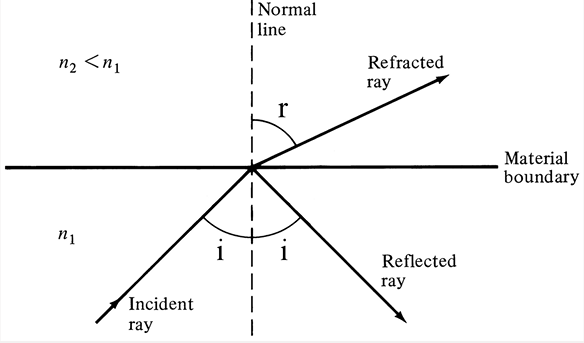
\includegraphics[width=0.5\linewidth]{FourAngles.png}}
	\key{Reflection:} part of the wave returns into the first medium, at the angle it arrived.\\
	\key{Refraction:} the transmitted part carries on with a new direction and a new speed.\\
	\key{Absorption:} the second medium may convert some of the energy to heat; in tissue this is wavelength-dependent.\\
	\key{Scattering:} a rough or inhomogeneous boundary sends light in many directions; tissue is a strong scatterer.\\
	Every sensor in this talk lives on the first two, and has to survive the last two.
\end{itemize}
\formula{\begin{aligned}
n&=\frac{c}{v},& \lambda_{\mathrm{medium}}&=\frac{\lambda_0}{n},& n_1\sin\theta_1&=n_2\sin\theta_2.
\end{aligned}}
\begin{itemize}
	\item Inside $n$ shows how much a medium slow light. $\Lambda_{medium}$ is the wavelength that shrinks inside the medium.
	\item Angles are measured from the normal. Reflection: \(\theta_r=\theta_i\). 
	Refraction bends at an index step; absorption and scattering reduce signal.
	\item And we use Fresnel reflection $R$ to quantify the fraction of light reflected at an interface.
\end{itemize}
\formula{\begin{aligned}
R&=\left(\frac{n_1-n_2}{n_1+n_2}\right)^2
\end{aligned}}
\begin{itemize}
	\item Beyond the critical angle, total internal reflection (TIR) confines light. 
	The evanescent field penetrates outside the guide and enables label-free sensing.
\end{itemize}

\subsection{Fibres and sensors}
\begin{itemize}
	\item The angle of refraction is usually determined by the refractive indices of the two media.
\end{itemize}
\formula{\mathrm{sin(\theta_c)=\frac{n_2}{n_1}}}
\begin{itemize}
	\item It valid only when \(n_1>n_2\). The critical angle is the minimum angle of incidence at which TIR occurs.
	\item Numerical aperture(NA) is a measure of the fibre's ability to collect light.
\end{itemize}
\formula{\mathrm{NA}=\sqrt{n_1^2-n_2^2},\qquad V=\frac{2\pi a}{\lambda}\mathrm{NA}}
\begin{itemize}
	\item Low \(V\) supports single-mode, clean phase for interferometry; high \(V\) supports multimode, 
	high collection but modal dispersion.
	\item Fibre loss: \(\alpha=\frac{10}{L}\log_{10}(\frac{P_{in}}{P_{out}})\) dB per length; 3 dB halves power.
	\item Sensing variables: intensity, phase, wavelength and polarization. Intrinsic sensors use the fibre itself; 
	extrinsic sensors use the fibre to reach an external transducer.
	\item A UV-written periodic index modulation reflects one narrow band and passes the rest. 
	And the Bragg wavelength is determined by the effective index and grating period.
\end{itemize}
\formula{\begin{aligned}
\lambda_B&=2n_{eff}\Lambda \cdot\frac{\Delta \lambda_B}{\lambda_B} &=(1-p_e)\epsilon+(\alpha+\zeta)\Delta T
\end{aligned}}

\formula{\begin{aligned}
\Delta\lambda&=S\,\Delta n, &\mathrm{FSR}&=\frac{\lambda^2}{n_gL}.
\end{aligned}}
\begin{itemize}
	\item FBG wavelength shifts report strain/temperature; use a reference grating for cross-sensitivity. 
	Ring resonators and Mach--Zehnder interferometers convert refractive-index changes to spectral or intensity shifts.
\end{itemize}

\subsection{Optical chip sensing}
\begin{itemize}
	\item Four ways of waveguide: slab(confined vertically), strip/channel, rib, buried.
	\item Platforms: silica-on-silicon (low loss), SiN (visible-capable, low loss), SOI (tight confinement) and polymers (cheap/printable).
	\item Grating coupler: wafer-testable, alignment-friendly, narrowband and polarization-sensitive. 
	Edge coupler: broadband/efficient, but needs polished facet and precise alignment.
	\item Specificity is chemistry, not optics: functionalize the sensing window, block the rest, and use a reference channel.
\end{itemize}

\subsection{Material selection}
\begin{center}\small
\begin{tabularx}{\linewidth}{@{}lYY@{}}
\toprule Material & Strength & Main use / risk\\ \midrule
Si & precise, stiff, wafer-scale & MEMS, moulds; opaque, brittle\\
Glass & transparent, chemical-stable & optics; brittle, costly bonding\\
Au/Pt & conductive, electrochemically useful & electrodes; corrosion/ion release\\
PDMS & clear, flexible, gas-permeable & prototypes/cells; absorption, swelling, evaporation\\
COC/COP & scalable, low absorption & disposable cartridges; tooling/bonding\\
Hydrogel & hydrated, tissue-like & 3D cell culture; swelling, weak mechanics\\
\bottomrule
\end{tabularx}\end{center}

\subsection{Fabrication backbone}
\begin{itemize}
	\item There are four core operations for fabricate biochips:\\
	\key{Clean \(\rightarrow\) deposit \(\rightarrow\) pattern \(\rightarrow\) etch \(\rightarrow\) 
	bond \(\rightarrow\) package \(\rightarrow\) test.}
	\item Deposition: CVD, PVD, sputtering, evaporation, spin coating. \\
	Patterning: photolithography, laser writing, nanoimprint, soft lithography. 
	Heat, plasma, UV, solvents and radiation may damage biomolecules/cells.
\end{itemize}


\section{4. Photolithography and Pattern Transfer}
\subsection{Principle}
\begin{itemize}
	\item The whole phtolithography mainly consists of 5 steps:\\
	\key{Light source:} generates exposing light, UV/visible light\\
	\key{Photomask:} selectively transmits light, define features\\
	\key{Photoresist:} changes chemistry on exposure, substrate coated with resist; exposure changes chemistry\\
	\key{Substrate:} receives the pattern, carries the resist-coated surface\\
	\key{Developer:} remove unwanted parts, removes newly soluble regions
\end{itemize}
\subsection{Standard flow}
\begin{enumerate}
	\item Clean substrate \(\rightarrow\) dehydration bake \(\rightarrow\) prime.
	\item Spin coat resist \(\rightarrow\) soft bake \(\rightarrow\) align mask and expose.
	\item Develop \(\rightarrow\) inspect/hard bake \(\rightarrow\) etch, deposit or mould.
	\item Strip temporary resist mask; bond or continue the process.
\end{enumerate}
\begin{itemize}
	\item While using spin coating, the resist thickness is controlled by viscosity and spin speed.
\end{itemize}
\formula{t\propto\frac{\eta^a}{\omega^b},\qquad D=It}
\begin{itemize}
	\item Inside \(t\) is resist thickness, \(\eta\) is resist viscosity, \(\omega\) is spin speed, 
	\(D\) is exposure dose, \(I\) is intensity and \(t\) is exposure time.
	\item Higher viscosity gives thicker resist; higher spin speed gives thinner film. 
	Exposure dose depends on intensity and time; 
	underexposure leaves incomplete transformation, overexposure enlarges/loses features.
\end{itemize}

\subsection{Resist and lithography}
\begin{itemize}
	\item \key{Positive resist:} becomes more soluble on exposure; produces same pattern as mask.
	\item \key{Negative resist:} becomes less soluble on exposure; produces inverse pattern of mask.\\
	\makebox[\linewidth][c]{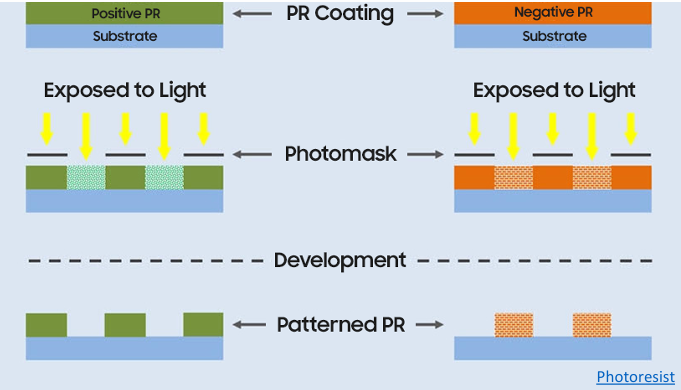
\includegraphics[width=0.5\linewidth]{Photoresist.png}}
\end{itemize}
\begin{center}\small
\begin{tabularx}{\linewidth}{@{}lYY@{}}
\toprule & Positive resist & Negative resist\\ \midrule
Exposed region & removed & remains\\
Chemistry & higher solubility & cross-linked/lower solubility\\
Typical use & fine etch patterns & thick moulds/structures\\
Risk & incomplete opening & residue/swelling\\
\bottomrule
\end{tabularx}\end{center}
\begin{itemize}
	\item Contact lithography has good resolution but can damage/contaminate the mask.
	\item Proximity reduces damage but adds diffraction.
	\item Projection gives high resolution/alignment at higher complexity and cost.
	\item Minimum feature size (CD) controls resolution:
\end{itemize}
\formula{\mathrm{CD}=k_1\frac{\lambda}{\mathrm{NA}}}
\begin{itemize}
	\item Smaller wavelength and larger NA improve resolution. 
	\item Reliability also requires alignment/overlay accuracy, throughput and dimensional control.
\end{itemize}

\subsection{Pattern transfer choices}
\begin{itemize}
	\item \key{Etching}: resist protects selected regions; exposed substrate is removed.
	\item \key{Lift-off}: pattern resist, deposit material, remove resist and unwanted film.
	\item \key{Replica moulding}: pattern master, cast polymer, cure and demould.
\end{itemize}


\section{5. Etching, Soft Lithography and PDMS}
\subsection{Etching definition}
\begin{itemize}
	\item \key{Definition:} Etching is the selective removal of material where the mask does not protect it.
	\item \key{Etch rate:} \(R=\) depth/time;
	\item \key{Selectivity:} \(S=R_{target}/R_{other}\);
	\item \key{Anisotropy} \(A=1-R_{lateral}/R_{vertical}\).
\end{itemize}

\subsection{Wet versus dry etching}
\begin{itemize}
	\item \key{Isotropic:} etche rate equally in all directions; rounded profile and undercut.
	\item \key{Anisotropic:} etche rate preferentially in one direction; sharp, sloped {111}, sidewalls.
\end{itemize}
\begin{center}\small
\begin{tabularx}{\linewidth}{@{}lYY@{}}
\toprule & Wet & Dry\\ \midrule
Mechanism & liquid chemistry & plasma radicals + ion sputtering\\
Profile & often isotropic/undercut & directional, near-vertical\\
Equipment & cheap, simple, fast & vacuum, complex, costly\\
Use & large areas, V-grooves & fine/high-aspect-ratio features\\
Risk & bubbles, chemical waste & plasma damage, resist erosion\\
\bottomrule
\end{tabularx}\end{center}
\begin{itemize}
	\item Isotropic etching removes equally in all directions: rounded profile and undercut.\\ 
	E.g. HNA (HF + HNO$_3$ + CH$_3$COOH) etches Si isotropically.
	\item KOH/TMAH anisotropically etch Si: on Si(100), {111} planes are slow and form \(54.74^\circ\) sidewalls/V-grooves.
	\item Dry etching requires volatile products. Reactive ion etching (RIE) combines chemical radicals and directional ion bombardment; 
	deep reactive ion etching(DRIE) gives deep vertical structures.\\
	E.g. Fluorine-based(S$F_6$, CF$_4$, CHF$_3$)etches Si/SiO$_2$/Si$_3$N$_4$, tends isotropic unless passivated; \\
	chlorine-based(Cl$_2$, BCl$_3$, HBr) etches metals, III–V semiconductors, polysilicon; tends anisotropic because needs ions.
\end{itemize}

\subsection{PDMS soft lithography}
\begin{itemize}
	\item PDMS is transparent, flexible, gas-permeable and inexpensive; it supports valves, microscopy and cell culture. \\
	Risks: hydrophobic-molecule absorption, solvent swelling, water evaporation, hydrophobic recovery and deformation.
\end{itemize}
\begin{enumerate}
	\item Make SU-8 master on Si.
	\item Mix PDMS base:curing agent = 10:1 by mass; degas.
	\item Pour and cure (typical \(65^\circ\mathrm C\), 2--4 h).
	\item Peel and punch inlets/outlets.
	\item O$_2$ plasma-treat PDMS and glass (roughly 30--90 s) and contact immediately.
	\item Attach tubing, fill and test for leakage/bubbles.
\end{enumerate}
\begin{itemize}
	\item \key{Common failures:} \\
	bubbles \(\rightarrow\) longer degas/slow pour; sticky PDMS \(\rightarrow\) verify 10:1 and cure; 
	sagging \(\rightarrow\) lower aspect ratio/cure harder; misaligned ports \(\rightarrow\) use a guide; 
	weak bond \(\rightarrow\) clean, activate both surfaces and bond promptly.
\end{itemize}

\subsection{Applications}
\begin{itemize}
	\item \key{Organ-on-chip:} uses perfusion, shear, co-culture and live imaging. 
	\item \key{Droplet microfluidics:} uses isolated picolitre reactors for digital PCR, single-cell analysis and enzyme evolution. 
	Low Re means mixing is diffusion-limited, not turbulent.
\end{itemize}


\section{6. Surface Engineering and Biointerfaces}
\subsection{Biointerface and assay background}
\begin{itemize}
	\item The biointerface is where material interacts with molecules, cells and fluids. For a low-abundance target in plasma:
\end{itemize}
\formula{\begin{aligned}
S_{measured}&=S_{specific}+S_{nonspecific}+S_{background}+S_{noise},\\
\mathrm{SBR}&\sim\frac{S_{specific}}{S_{nonspecific}+S_{background}}.
\end{aligned}}
\begin{itemize}
	\item The surface must capture selectively, suppress fouling, preserve recognition-site access and survive washing/storage.
\end{itemize}

\subsection{Protein adsorption and fouling}
Adsorption sequence: transport \(\rightarrow\) contact \(\rightarrow\) reorientation \(\rightarrow\) conformational change \(\rightarrow\) reversible/stable attachment. Drivers include hydrophobic, electrostatic, hydrogen-bond, van der Waals, entropic and affinity interactions.
\begin{itemize}
	\item \key{Specific binding}: intended target-recognition event.
	\item \key{Nonspecific adsorption}: unintended molecule/cell attachment.
	\item \key{Biofouling}: broader unwanted biological accumulation.
	\item Fouling causes high blank, blocked sites, reduced sensitivity, drift, poor reproducibility and channel blockage.
	\item \key{Vroman effect}: abundant proteins arrive first; later high-affinity proteins can displace/reorient them over time.
\end{itemize}

\subsection{Wettability and surface energy}
\begin{itemize}
	\item Contact angle \(\theta\) is measured through the liquid at the solid--liquid--vapor line. \(\theta<90^\circ\): hydrophilic; \(\theta>90^\circ\): hydrophobic.
	\item Wettability affects channel filling, droplet spreading, reagent delivery, functionalization, cell attachment and reproducibility. Contact angle alone does not prove low protein adsorption.
	\item Surface energy is excess molecular energy at the surface; it affects wetting, adhesion, coating attachment, adsorption and cell attachment.
\end{itemize}

\subsection{Surface modification}
\begin{itemize}
	\item \key{O$_2$ plasma}: removes contamination, adds --OH/--C=O/--COOH, raises surface energy and improves wetting/bonding; risk: nonuniformity, damage and hydrophobic recovery.
	\item \key{Silanization}: oxide surface --OH reacts with silane. APTES gives amine, GPTMS epoxy, MPTMS thiol termination.
	\item \key{SAM}: organized layer controlled by substrate, binding group, spacer, terminal chemistry, defects and packing.
	\item \key{Thiol--Au}: \(\mathrm{Au+RSH\rightarrow Au-S-R}\); useful for DNA, peptides and electrochemical interfaces.
	\item \key{PEG/polymer brushes}: hydration + steric repulsion reduce adsorption; incomplete coverage, degradation and blocked target access are risks.
	\item Hydrogels give hydrated 3D interfaces but may swell and limit diffusion; layer-by-layer films tune thickness, charge and composition.
\end{itemize}

\subsection{Biomolecule immobilization}
\begin{center}\small
\scriptsize\begin{tabularx}{\linewidth}{@{}lYY@{}}
\toprule Method & Strength / benefit & Main limitation\\ \midrule
Physical adsorption & simple, gentle & weak, leaching, poor orientation\\
EDC/NHS covalent & stable, wash-resistant & random orientation, activity loss\\
Thiol--Au & strong, defined on gold & substrate-specific\\
Biotin--streptavidin & high affinity, modular & extra chemistry / background\\
Fc-oriented antibody & accessible Fab sites & implementation depends\\
\bottomrule
\end{tabularx}\end{center}
\begin{itemize}
	\item \key{Universal criteria}: strong attachment, retained activity, accessible binding sites, low background, 
	reproducibility and detector compatibility. Cell adhesion depends on ECM ligands (e.g. RGD/collagen), 
	charge/chemistry, stiffness, topography, ligand density and shear.
\end{itemize}

\section*{High-yield contrasts}
\begin{itemize}
	\item Integration connects functions; automation removes manual steps.
	\item Low Re means laminar, not automatically well-mixed; diffusion time scales as \(L^2\).
	\item Low Pe favours diffusion; high Pe favours downstream advection.
	\item Isotropic etch rounds/undercuts; anisotropic Si etch follows crystal planes.
	\item Wet etch is simple/cheap; dry etch is directional/high-aspect-ratio.
	\item Photolithography defines a temporary resist mask; etching creates the lasting structure.
	\item Plasma activates PDMS but the surface recovers hydrophobicity with time.
	\item Hydrophilic does not equal antifouling; a low-fouling layer must still expose the recognition element.
	\item Optics supplies sensitivity; surface chemistry supplies specificity.
\end{itemize}

\end{multicols*}
\end{document}
